% ===================== PARTE I: PANORAMICA =====================
\part{Come funziona il progetto}

\section{Il problema}

La \textbf{visual saliency prediction} consiste nel predire quali zone di un'immagine attirano
l'attenzione visiva di un osservatore umano. L'output è una \emph{saliency map}: un'immagine in
scala di grigi dove il valore di ogni pixel indica quanta attenzione quel punto riceve.

NOVA confronta più modelli di saliency valutandoli contro una ground truth costruita con
\textbf{click del mouse come proxy del gaze}. Come passo finale, le saliency map vengono
combinate con dei bounding box per produrre un \textbf{ranking degli oggetti} per importanza
visiva.

\begin{nota}
\textbf{Perché i click e non un eye-tracker.} Un eye-tracker è costoso e non disponibile. La
soluzione adottata non è un ripiego improvvisato: è il metodo con cui è stato costruito
\textbf{SALICON}, uno dei dataset di riferimento della letteratura. Chiedendo a una persona di
cliccare sui punti che attirano la sua attenzione si ottiene una distribuzione spaziale
fortemente correlata con quella delle fissazioni oculari reali.
\end{nota}

\subsection{Input e output}

\begin{center}
\begin{tabular}{l p{10.4cm}}
\toprule
\rowcolor{tblHead}\textcolor{white}{\textbf{}} & \textcolor{white}{\textbf{}} \\
\midrule
\textbf{Input} & Una singola immagine RGB \\
\rowcolor{tblAlt} \textbf{Output 1} & Una saliency map per ciascun modello: \pyin{float32}, valori in $[0,1]$, stesse dimensioni dell'immagine \\
\textbf{Output 2} & Una lista di oggetti ordinati per importanza visiva predetta \\
\rowcolor{tblAlt} \textbf{Output 3} & Tabelle di metriche che quantificano l'accordo di ogni modello con la ground truth \\
\bottomrule
\end{tabular}
\end{center}

\section{La pipeline}

\begin{idebox}
\begin{Verbatim}[commandchars=\\\{\},fontsize=\footnotesize]
\textcolor{ideComment}{[1] RACCOLTA}
    \textcolor{ideFg}{foto in prima persona}  ──►  \textcolor{ideFunc}{data/eval/}

\textcolor{ideComment}{[2] ANNOTAZIONE}                                    \textcolor{ideComment}{annotate.py}
    \textcolor{ideFg}{click ordinati (3-6 per immagine, più annotatori)}
                            │
                            ▼
                  \textcolor{ideFunc}{data/annotations/*.json}

\textcolor{ideComment}{[3] GROUND TRUTH}                          \textcolor{ideComment}{ground_truth.py}
    \textcolor{ideFg}{click}  ──┬──►  \textcolor{ideFunc}{mappa di fissazione}   \textcolor{ideComment}{(binaria)}
             └──►  \textcolor{ideFunc}{heatmap continua}      \textcolor{ideComment}{(Gaussiane sommate)}

\textcolor{ideComment}{[4] PREDIZIONE}                              \textcolor{ideComment}{registry.py}
    \textcolor{ideFg}{immagine}  ──►  \textcolor{ideFunc}{Center Prior / Spectral Residual / Itti-Koch}
                            │
                            ▼
                     \textcolor{ideFunc}{saliency map}

\textcolor{ideComment}{[5] CONFRONTO}                                 \textcolor{ideComment}{metrics.py}
    \textcolor{ideFg}{saliency map  vs  ground truth}
                            │
                            ▼
              \textcolor{ideFunc}{CC, SIM, KL, NSS, AUC-Judd}

\textcolor{ideComment}{[6] RANKING}                                   \textcolor{ideComment}{objects.py}
    \textcolor{ideFg}{saliency + box}  ──►  \textcolor{ideFunc}{ranking predetto}
    \textcolor{ideFg}{click + box}     ──►  \textcolor{ideFunc}{ranking di riferimento}
                            │
                            ▼
            \textcolor{ideFunc}{Spearman, Kendall, Top-1}
\end{Verbatim}
\end{idebox}

\subsection{Un esempio concreto}

\begin{center}
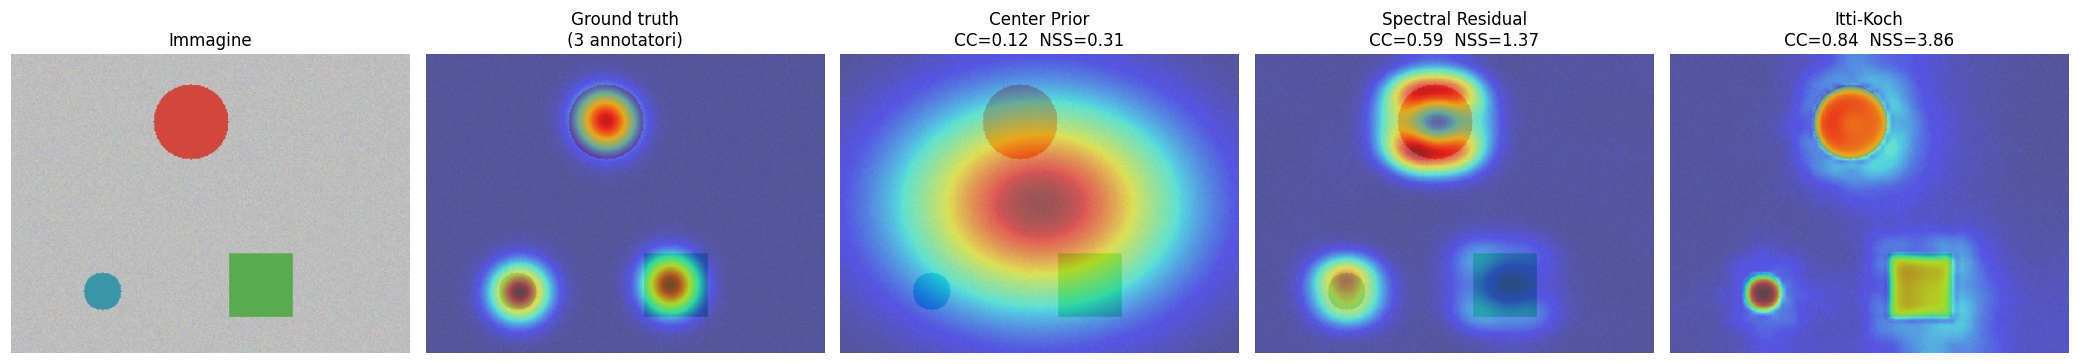
\includegraphics[width=\textwidth]{pipeline_example.png}
\end{center}

Da sinistra: l'immagine, la ground truth costruita dai click di tre annotatori, e le predizioni
dei tre modelli con le rispettive metriche. Si vede il progresso: il center prior illumina il
centro ignorando gli oggetti, Spectral Residual li individua parzialmente, Itti-Koch li coglie
tutti e tre.

\section{L'architettura}

\subsection{I tre livelli}

\begin{center}
\begin{tabular}{l p{8.8cm}}
\toprule
\rowcolor{tblHead}\textcolor{white}{\textbf{Livello}} & \textcolor{white}{\textbf{Responsabilità}} \\
\midrule
\texttt{src/baselines/} & I modelli: immagine $\to$ saliency map \\
\rowcolor{tblAlt} \texttt{src/registry.py} & Uniformare l'accesso ai modelli \\
\texttt{src/visualization.py} & Saliency map $\to$ immagine guardabile \\
\rowcolor{tblAlt} \texttt{app.py}, \texttt{annotate.py} & Solo interfaccia: layout ed eventi \\
\bottomrule
\end{tabular}
\end{center}

\begin{nota}
\textbf{Perché non scrivere tutto in \texttt{app.py}.} Sarebbe più corto e funzionerebbe
identicamente, ma: (1) un'interfaccia grafica non si testa automaticamente, la logica sotto sì;
(2) gli script di valutazione riuserebbero le stesse funzioni, che andrebbero duplicate; (3)
aggiungere un modello richiederebbe di toccare più punti invece di uno solo.
\end{nota}

\subsection{Il contratto della saliency map}

Tutti i modelli rispettano lo stesso contratto di uscita:

\begin{center}
\begin{tabular}{>{\bfseries}l l}
\toprule
\rowcolor{tblHead}\textcolor{white}{\textbf{Proprietà}} & \textcolor{white}{\textbf{Valore}} \\
\midrule
Tipo & \pyin{np.float32} \\
\rowcolor{tblAlt} Range & $[0, 1]$ --- 0 = ignorato, 1 = massima attenzione \\
Dimensioni & identiche a \pyin{(height, width)} dell'input \\
\bottomrule
\end{tabular}
\end{center}

Deciso una volta e valido per tutti. Se ogni modello restituisse un formato diverso servirebbero
conversioni sparse in tutto il codice, con rischio concreto di confronti falsati.

\subsection{La convenzione BGR}

OpenCV carica le immagini in ordine \textbf{BGR}, non RGB. Tutto il progetto adotta questa
convenzione; la conversione a RGB avviene solo al momento di visualizzare.

\begin{attenzione}
\textbf{Errore silenzioso da conoscere.} Passare un'immagine RGB a una funzione che si aspetta
BGR non solleva nessuna eccezione: la forma è giusta e l'immagine resta visualizzabile.
Semplicemente rosso e blu sono scambiati --- e Itti-Koch, che ha canali di opponenza cromatica,
produce risultati sbagliati senza alcun segnale.
\end{attenzione}

\section{Struttura dei file}

\begin{idebox}
\begin{Verbatim}[commandchars=\\\{\},fontsize=\footnotesize]
\textcolor{ideFunc}{app.py}                   \textcolor{ideComment}{interfaccia web di confronto}
\textcolor{ideFunc}{annotate.py}              \textcolor{ideComment}{interfaccia web di annotazione}
\textcolor{ideFunc}{requirements.txt}
\textcolor{ideFunc}{src/}
├── \textcolor{ideFg}{registry.py}          \textcolor{ideComment}{registro centrale dei modelli}
├── \textcolor{ideFg}{visualization.py}     \textcolor{ideComment}{heatmap, overlay, marcatori}
├── \textcolor{ideFunc}{baselines/}
│   ├── \textcolor{ideFg}{center_prior.py}       \textcolor{ideComment}{baseline: Gaussiana centrata}
│   ├── \textcolor{ideFg}{spectral_residual.py}  \textcolor{ideComment}{FFT + residuo spettrale}
│   └── \textcolor{ideFg}{itti_koch.py}          \textcolor{ideComment}{center-surround multi-scala}
├── \textcolor{ideFunc}{annotation/}
│   ├── \textcolor{ideFg}{store.py}              \textcolor{ideComment}{persistenza delle annotazioni}
│   └── \textcolor{ideFg}{ground_truth.py}       \textcolor{ideComment}{click -> heatmap e fissazioni}
├── \textcolor{ideFunc}{evaluation/}
│   └── \textcolor{ideFg}{metrics.py}            \textcolor{ideComment}{tutte le metriche}
└── \textcolor{ideFunc}{ranking/}
    └── \textcolor{ideFg}{objects.py}            \textcolor{ideComment}{ranking degli oggetti}
\textcolor{ideFunc}{scripts/run_evaluation.py} \textcolor{ideComment}{valutazione -> tabelle CSV}
\textcolor{ideFunc}{tests/test_all.py}         \textcolor{ideComment}{56 controlli}
\end{Verbatim}
\end{idebox}

\subsection{Comandi}

\begin{idebox}
\begin{bashcode}
python3 -m venv venv
source venv/bin/activate          # Windows: venv\Scripts\activate
pip install -r requirements.txt

python app.py                     # interfaccia di confronto
python annotate.py --images data/eval   # interfaccia di annotazione
python scripts/run_evaluation.py  # valutazione completa
python tests/test_all.py          # 56 test
\end{bashcode}
\end{idebox}

\newpage

% ===================== PARTE II: FILE PER FILE =====================
\part{Il codice, file per file}

I file sono presentati in \textbf{ordine di dipendenza}: prima quelli che non dipendono da
nessuno, poi quelli che li usano. Leggendoli in quest'ordine non si incontra mai un riferimento
a qualcosa non ancora spiegato.

\section{\texttt{src/baselines/center\_prior.py}}

Il modello più semplice del progetto, e il punto migliore da cui iniziare a leggere il codice.

\subsection{A cosa serve}

Genera una Gaussiana 2D fissa al centro dell'immagine, \textbf{ignorando completamente il
contenuto}. A parità di dimensioni restituisce sempre la stessa identica mappa.

\begin{nota}
\textbf{Perché una baseline così banale è indispensabile.} Nella letteratura sull'attenzione
visiva è documentato il \emph{center bias}: le persone guardano il centro di una scena molto più
spesso della periferia, sia perché chi scatta tende a inquadrare al centro il soggetto, sia per
una tendenza oculomotoria naturale.

\medskip
Un modello che non batte questa Gaussiana non sta estraendo \emph{nessuna} informazione
dall'immagine: sta solo riscoprendo il center bias. Le linee guida del corso richiedono
esplicitamente almeno una baseline, e questa è la scelta standard per la saliency.
\end{nota}

\subsection{La firma}

\begin{idebox}
\begin{pycode}
def center_prior_saliency(image_shape, sigma_frac=0.25):
\end{pycode}
\end{idebox}

\begin{center}
\begin{tabular}{>{\ttfamily}l l p{6.9cm}}
\toprule
\rowcolor{tblHead}\textcolor{white}{\textbf{Parametro}} & \textcolor{white}{\textbf{Tipo}} & \textcolor{white}{\textbf{Significato}} \\
\midrule
image\_shape & tuple(int,int) & \pyin{(altezza, larghezza)}. Si passa la \emph{forma}, non l'immagine. \\
\rowcolor{tblAlt} sigma\_frac & float & Deviazione standard come frazione delle dimensioni. \\
\bottomrule
\end{tabular}
\end{center}

\begin{nota}
\textbf{Perché la firma accetta la forma e non l'immagine.} È una scelta deliberata di
\emph{design comunicativo}: la firma stessa dichiara che il modello non guarda mai il contenuto.
Accettare l'immagine e poi ignorarla sarebbe funzionalmente identico ma fuorviante per chi legge
il codice.
\end{nota}

\subsection{Il corpo, riga per riga}

\subsubsection{Centro e deviazioni standard}

\begin{idebox}
\begin{pycode}
height, width = image_shape

cx = width / 2.0
cy = height / 2.0
sigma_x = sigma_frac * width
sigma_y = sigma_frac * height
\end{pycode}
\end{idebox}

\pyin{cx} e \pyin{cy} sono le coordinate del centro geometrico. La divisione è per \pyin{2.0}
(float) e non per \pyin{2} (int) per evitare la divisione intera su immagini di dimensione
dispari.

\pyin{sigma_x} e \pyin{sigma_y} sono \textbf{separati e proporzionali} alle rispettive
dimensioni. Con un unico $\sigma$ espresso in pixel:

\begin{itemize}
  \item su un'immagine 320$\times$240 la macchia coprirebbe una frazione diversa della larghezza
  rispetto all'altezza --- un'ellisse schiacciata rispetto alla forma dell'immagine;
  \item la stessa scena a risoluzione 4K avrebbe una macchia relativamente minuscola.
\end{itemize}

\subsubsection{La griglia di coordinate}

\begin{idebox}
\begin{pycode}
x = np.arange(width, dtype=np.float32)
y = np.arange(height, dtype=np.float32)
xx, yy = np.meshgrid(x, y)
\end{pycode}
\end{idebox}

\pyin{np.arange(width)} produce il vettore $[0, 1, 2, \ldots, \text{width}-1]$.
\pyin{np.meshgrid} li combina in due matrici delle dimensioni dell'immagine:

\begin{itemize}
  \item \pyin{xx[i, j] == j} --- la coordinata orizzontale (colonna) di ogni pixel;
  \item \pyin{yy[i, j] == i} --- la coordinata verticale (riga) di ogni pixel.
\end{itemize}

Avendo le coordinate come matrici, la Gaussiana si calcola su tutti i pixel in \emph{una sola}
operazione vettorizzata, senza cicli \pyin{for} annidati --- che in Python sarebbero ordini di
grandezza più lenti.

\begin{attenzione}
\textbf{Trappola di indicizzazione.} In numpy il primo indice è la \emph{riga} ($y$), il secondo
la \emph{colonna} ($x$): si scrive \pyin{img[y, x]}. È l'inverso della notazione matematica
$(x, y)$. Praticamente tutti gli scambi $x$/$y$ in questo progetto nascono da qui.
\end{attenzione}

\subsubsection{La Gaussiana}

\begin{idebox}
\begin{pycode}
exponent = -((xx - cx) ** 2 / (2.0 * sigma_x ** 2)
             + (yy - cy) ** 2 / (2.0 * sigma_y ** 2))
gauss = np.exp(exponent)
\end{pycode}
\end{idebox}

Implementazione diretta della Gaussiana 2D separabile:
\[
G(x,y) = \exp\!\left(-\left[\frac{(x-c_x)^2}{2\sigma_x^2} + \frac{(y-c_y)^2}{2\sigma_y^2}\right]\right)
\]

L'esponente è calcolato separatamente per leggibilità. Il valore massimo è $1.0$, raggiunto
esattamente al centro dove entrambi i termini si annullano.

\subsubsection{La normalizzazione}

\begin{idebox}
\begin{pycode}
def _normalize(saliency_map):
    minimum, maximum = saliency_map.min(), saliency_map.max()
    if maximum - minimum > 0:
        saliency_map = (saliency_map - minimum) / (maximum - minimum)
    else:
        saliency_map = np.zeros_like(saliency_map)
    return saliency_map.astype(np.float32)
\end{pycode}
\end{idebox}

Normalizzazione \emph{min-max}: sottrae il minimo e divide per l'escursione, portando i valori
in $[0,1]$.

\begin{nota}
\textbf{Perché normalizzare se il massimo è già 1.0.} Tre motivi: (1) il minimo non è
necessariamente 0, quindi il range va comunque riscalato; (2) rende il contratto identico a
quello degli altri modelli, dove la normalizzazione è indispensabile; (3) il ramo \pyin{else}
protegge dal caso degenere di mappa costante --- qui non può accadere, ma negli altri modelli sì,
e avere lo stesso schema ovunque riduce il rischio di dimenticarlo dove serve.
\end{nota}

Il prefisso \pyin{_} nel nome segnala che è una funzione interna al modulo, non parte
dell'interfaccia pubblica.

\section{\texttt{src/baselines/spectral\_residual.py}}

Riferimento: Hou \& Zhang, \emph{Saliency Detection: A Spectral Residual Approach}, CVPR 2007.

\subsection{L'idea}

Le immagini naturali, mediamente, hanno uno spettro di ampiezza molto regolare: le basse
frequenze dominano e l'energia decade in modo prevedibile al crescere della frequenza. Questa
regolarità è la parte \textbf{ridondante} di una scena --- ciò che tutte le immagini hanno in
comune.

L'ipotesi del metodo: \emph{ciò che devia dall'andamento atteso è l'informazione interessante}.
Si stima l'andamento atteso sfocando il logaritmo dello spettro, lo si sottrae, e ciò che resta
--- il \textbf{residuo spettrale} --- indica le frequenze statisticamente anomale.

\begin{nota}
\textbf{Perché funziona pur essendo ``solo'' un trucco statistico.} Un oggetto saliente ha
tipicamente bordi netti, una texture diversa dallo sfondo, una forma compatta: tutte
caratteristiche che producono energia a frequenze non generiche rispetto al resto della scena.
Il metodo non capisce cosa sia un oggetto, ma la statistica è un buon sostituto --- e costa circa
trenta righe di codice, senza alcun addestramento.
\end{nota}

\subsection{La pipeline in sette passi}

\subsubsection{Passo 1 --- Scala di grigi}

\begin{idebox}
\begin{pycode}
original_h, original_w = image.shape[:2]

if image.ndim == 3 and image.shape[2] == 3:
    gray = cv2.cvtColor(image, cv2.COLOR_BGR2GRAY)
else:
    gray = image.copy()
\end{pycode}
\end{idebox}

Le dimensioni originali si salvano \emph{subito}: serviranno alla fine per riportare la mappa
alla risoluzione di partenza.

Il controllo \pyin{image.ndim == 3 and image.shape[2] == 3} rende la funzione tollerante: accetta
sia immagini a colori sia già in scala di grigi. Il \pyin{.copy()} nel ramo \pyin{else} evita di
lavorare sullo stesso array passato dal chiamante.

\begin{attenzione}
Questo passo è la causa del limite più importante del metodo: \textbf{l'informazione cromatica
viene distrutta}. Un oggetto che si distingue solo per tinta ma non per luminosità diventa
invisibile al modello. Il fenomeno è verificato numericamente nella sezione dei test.
\end{attenzione}

\subsubsection{Passo 2 --- Riduzione di risoluzione}

\begin{idebox}
\begin{pycode}
small = cv2.resize(gray, target_size,
                   interpolation=cv2.INTER_AREA).astype(np.float32)
\end{pycode}
\end{idebox}

Il default \pyin{target_size=(64, 64)} è il valore del paper originale. La saliency è un fenomeno
a bassa frequenza spaziale --- interessa \emph{dove} guardare, non i dettagli fini --- quindi
lavorare a piena risoluzione non aggiunge informazione e costa molto di più.

\pyin{INTER_AREA} è l'interpolazione corretta per \emph{rimpicciolire}: calcola la media dei
pixel dell'area sorgente che confluisce in ogni pixel destinazione. Le alternative
(\pyin{INTER_LINEAR}, \pyin{INTER_NEAREST}) campionano pochi pixel e producono
\emph{aliasing} --- artefatti ad alta frequenza che qui sarebbero disastrosi, dato che il metodo
analizza proprio lo spettro delle frequenze.

Il cast a \pyin{float32} è necessario prima della FFT: su \pyin{uint8} i calcoli andrebbero in
overflow.

\subsubsection{Passo 3 --- FFT e separazione ampiezza/fase}

\begin{idebox}
\begin{pycode}
spectrum = np.fft.fft2(small)
amplitude = np.abs(spectrum)
phase = np.angle(spectrum)
\end{pycode}
\end{idebox}

\pyin{np.fft.fft2} produce una matrice di numeri \emph{complessi}. Ogni numero complesso
$z = a + bi$ si può leggere in forma polare come $z = |z| e^{i\theta}$:

\begin{itemize}
  \item \pyin{np.abs(spectrum)} $= |z|$ --- l'\textbf{ampiezza}: \emph{quanta} energia c'è a
  quella frequenza;
  \item \pyin{np.angle(spectrum)} $= \theta$ --- la \textbf{fase}: \emph{dove} sono posizionate
  le strutture nell'immagine.
\end{itemize}

\subsubsection{Passo 4 --- Il residuo}

\begin{idebox}
\begin{pycode}
log_amplitude = np.log(amplitude + 1e-8)
avg_log_amplitude = cv2.blur(log_amplitude, (3, 3))
spectral_residual = log_amplitude - avg_log_amplitude
\end{pycode}
\end{idebox}

Tre righe, tre decisioni:

\begin{description}[leftmargin=1.2em,style=nextline]
\item[\pyin{np.log(...)}] L'ampiezza varia di diversi ordini di grandezza tra basse e alte
frequenze. Il logaritmo comprime questo range, rendendo l'andamento generale approssimabile con
una semplice media locale.

\item[\pyin{+ 1e-8}] Protezione da $\log(0)$, che darebbe $-\infty$ e propagherebbe NaN in tutto
il calcolo. Il valore è abbastanza piccolo da non alterare i risultati.

\item[\pyin{cv2.blur(..., (3,3))}] Filtro a media mobile: stima l'andamento ``atteso'' dello
spettro. La differenza tra spettro reale e atteso è il \textbf{residuo}, cioè la parte
statisticamente anomala.
\end{description}

\subsubsection{Passo 5 --- Ricostruzione}

\begin{idebox}
\begin{pycode}
reconstructed = np.fft.ifft2(np.exp(spectral_residual + 1j * phase))
saliency = (np.abs(reconstructed) ** 2).astype(np.float32)
\end{pycode}
\end{idebox}

Riga densa, va letta dall'interno verso l'esterno:

\begin{enumerate}
  \item \pyin{spectral_residual + 1j * phase} --- ricompone un numero complesso usando il residuo
  come parte reale (siamo nel dominio logaritmico) e la fase \textbf{originale} come parte
  immaginaria. \pyin{1j} è l'unità immaginaria in Python.
  \item \pyin{np.exp(...)} --- annulla il logaritmo del passo 4, tornando al dominio lineare.
  \item \pyin{np.fft.ifft2(...)} --- FFT inversa: dal dominio delle frequenze allo spazio
  immagine.
  \item \pyin{np.abs(...) ** 2} --- modulo al quadrato, cioè l'\emph{energia}. Sempre positiva,
  come deve essere una saliency map.
\end{enumerate}

\begin{nota}
\textbf{Perché si conserva la fase originale.} Il metodo modifica solo l'ampiezza. Se si
scartasse la fase e se ne usasse una casuale, la ricostruzione non avrebbe alcuna relazione
spaziale con la scena: si otterrebbe rumore. La fase è ciò che àncora l'informazione alla
posizione.
\end{nota}

\subsubsection{Passo 6 --- Smoothing}

\begin{idebox}
\begin{pycode}
ksize = int(np.ceil(sigma * 6)) | 1
saliency = cv2.GaussianBlur(saliency, (ksize, ksize), sigma)
\end{pycode}
\end{idebox}

\pyin{cv2.GaussianBlur} richiede una dimensione di kernel \emph{dispari}.

\begin{description}[leftmargin=1.2em,style=nextline]
\item[\pyin{sigma * 6}] Regola pratica: una Gaussiana è praticamente nulla oltre $\pm 3\sigma$,
quindi un kernel di $6\sigma$ la contiene quasi interamente.
\item[\pyin{| 1}] OR bit-a-bit con 1: forza a 1 il bit meno significativo, trasformando qualsiasi
numero pari nel dispari successivo ($12 \to 13$, $13 \to 13$). Idioma compatto per ``arrotonda al
dispari''.
\end{description}

Lo smoothing non è cosmetico: la ricostruzione grezza è molto puntinata, mentre l'attenzione
umana si concentra su \emph{regioni}, non su singoli pixel isolati.

\subsubsection{Passo 7 --- Ritorno alla risoluzione originale}

\begin{idebox}
\begin{pycode}
saliency = _normalize(saliency)
return cv2.resize(saliency, (original_w, original_h),
                  interpolation=cv2.INTER_LINEAR)
\end{pycode}
\end{idebox}

Qui si usa \pyin{INTER_LINEAR} perché si sta \emph{ingrandendo}, il caso opposto al passo 2.

\begin{attenzione}
\pyin{cv2.resize} vuole la dimensione come \pyin{(width, height)}, mentre \pyin{shape} di numpy è
\pyin{(height, width)}. L'ordine invertito è una fonte classica di bug silenziosi: l'immagine
esce distorta senza alcun errore.
\end{attenzione}
